% !TEX encoding = UTF-8 Unicode
\documentclass[a4paper]{article}

% Dodato da se ne bi prikazivali podnaslovi u sadrzaju, a da ipak ostanu numerisani u okviru teksta
%\setcounter{tocdepth}{1}    % levels under \subsection are not listed in the TOC


\usepackage{color}
\usepackage{url}
\usepackage[utf8]{inputenc} % make weird characters work
\usepackage{graphicx}


\usepackage[english,serbian]{babel}

\usepackage[unicode]{hyperref}
\hypersetup{colorlinks,citecolor=green,filecolor=green,linkcolor=blue,urlcolor=blue}

\usepackage{listings}
\usepackage{amsmath,amssymb}

\newtheorem{primer}{Primer}[section]

\definecolor{mygreen}{rgb}{0,0.6,0}
\definecolor{mygray}{rgb}{0.7,0.7,0.7}
\definecolor{mymauve}{rgb}{0.58,0,0.82}

\lstset{ 
  backgroundcolor=\color{white},   % choose the background color; you must add \usepackage{color} or \usepackage{xcolor}; should come as last argument
  basicstyle=\scriptsize\ttfamily,        % the size of the fonts that are used for the code
  breakatwhitespace=false,         % sets if automatic breaks should only happen at whitespace
  breaklines=false,                 % sets automatic line breaking
  captionpos=b,                    % sets the caption-position to bottom
  commentstyle=\color{mygreen},    % comment style
  deletekeywords={...},            % if you want to delete keywords from the given language
  escapeinside={\%*}{*)},          % if you want to add LaTeX within your code
  extendedchars=true,              % lets you use non-ASCII characters; for 8-bits encodings only, does not work with UTF-8
%  firstnumber=1000,                % start line enumeration with line 1000
  frame=single,	                   % adds a frame around the code
  keepspaces=true,                 % keeps spaces in text, useful for keeping indentation of code (possibly needs columns=flexible)
  keywordstyle=\color{blue},       % keyword style
  language=Python,                 % the language of the code
  morekeywords={*,...},            % if you want to add more keywords to the set
%  numbers=left,                    % where to put the line-numbers; possible values are (none, left, right)
%  numbersep=0pt,                   % how far the line-numbers are from the code
%  numberstyle=\tiny\color{mygray}, % the style that is used for the line-numbers
  rulecolor=\color{black},         % if not set, the frame-color may be changed on line-breaks within not-black text (e.g. comments (green here))
  showspaces=false,                % show spaces everywhere adding particular underscores; it overrides 'showstringspaces'
  showstringspaces=false,          % underline spaces within strings only
  showtabs=false,                  % show tabs within strings adding particular underscores
%  stepnumber=2,                    % the step between two line-numbers. If it's 1, each line will be numbered
  stringstyle=\color{mymauve},     % string literal style
  tabsize=2,	                   % sets default tabsize to 2 spaces
  title=\lstname                   % show the filename of files included with \lstinputlisting; also try caption instead of title
}

\renewcommand{\lstlistingname}{Kod}% Listing -> Algorithm
\renewcommand{\lstlistlistingname}{List of \lstlistingname s}%

\begin{document}

\title{Prepoznavanje saobraćajnih znakova pomoću konvolutivnih neuronskih mreža\\ \small{Seminarski rad u okviru kursa\\Računarska inteligencija\\ Matematički fakultet}}

\author{Jana Jovičić 215/2015, Jovana Pejkić 435/2016 \\ jana.jovicic755@gmail.com, jov4ana@gmail.com}

\date{16.~maj 2019.}

\maketitle

\abstract{

}

\newpage

\tableofcontents

\newpage

\section{Uvod}
\label{sec:uvod}

Prepoznavanje i klasifikacija slika je polje u oblasti mašinskog učenja koje se veoma brzo razvija. Na primer, klasifikatori slika se sve više koristite za: zamenu lozinke prepoznavanjem lica, prepoznavanje otisaka prstiju, analizu krvnih slika, identifikaciju geografskih karakteristika iz satelitskih snimaka, analizu aero i satelitskih snimaka, detekciju urbanih područja, detekciju puteva, autonomnu vožnju i otkrivanje prepreka itd.

Klasifikacija je vrsta problema nadgledanog učenja\footnote{Nadgledano učenje (eng. supervised learning) je proces učenja funkcije koja preslikava ulaz u odgovarajući izlaz, zasnovan na datim ulzno-izlaznim parovima. Dve osnovne vrste problema nadgledanog učenja su regresija i klasifikacija. Regresija je problem predvidanja neprekidne, a klasifikacija kategoričke ciljne promenljive.} koja podrazumeva predviđanje kategoričke ciljne promenljive. Kategoričkim se smatraju promenljive koje uzimaju konačan broj vrednosti (među kojima nema uređenja). Na primer, prepoznavanje da li je dobijen e-mail \textit{smeće (eng.} spam\textit{)}, reklama ili obična poruka je problem klasifikacije.

Postoje mnogi algoritmi koji se koriste za klasifikaciju slika (npr. SVM\footnote{\textit{Podržavajući vektori (eng.} Support vector machines SVM\textit{)} predstavljaju model nadgledanog učenja koji se koristi za klasifikacionu i regresionu analizu.}), a jedan od najboljih predstavljaju \textit{konvolutivne neuronske mreže (eng.} convolutional neural network, CNN\textit{)}. CNN se može zamisliti kao automatski ‚‚ekstraktor’’ karakteristika slike. On efikasno koristi informacije o susednim pikselima kako bi konvolucijom i agregacijom smanjio sliku, a zatim predvideo kategoriju kojoj slika pripada. Iako su konvolutivne neuronske mreže projektovane tako da prednost postižu u radu sa 2D strukturama, kao što su slike ili ulazi poput \textit{govornog signala (eng.} speech signal\textit{)}, najnovije studije pokazuju da postižu značajne rezultate i sa 3D strukturama.

U ovom radu je predstavljeno rešavanje problema klasifikacije slika saobraćajnih znakova pomoću neuronskih mreža (koje su opisane u poglavlju \ref{sec:neuronske_mreze}), i to konvolutivnih neuronskih mreža (koje su opisane u poglavlju \ref{sec:cnn}). Cilj ovog rada je da, kroz rešavanje ovog problema, prikaže osnovne osobine konvolutivnih neuronskih mreža kao i njihovu implementaciju. U radu je, u poglavlju \ref{sec:implementacija_i_eksperimentalni_rezultati}, najpre opisano nekoliko razlicitih modela mreža, a onda su upoređeni i analizirani ostvareni rezultati.


% TODO TODO TODO rec nekoliko u poslednjoj recenici zameniti sa tacnim brojem modela u radu!

\newpage

\section{Neuronske mreže}
\label{sec:neuronske_mreze}

%U masinskom učenju, neuronske mreže (eng. neural networks) važe za jednu od najprimenjenijih metoda.
Neuronske mreže predstavljaju skup statističkih modela učenja inspirisana biološkim neuronima, za rešavanje klasifikacionih\footnote{Klasifikacioni problem - ako je izlazna promenljiva kategorickog tipa, npr. ,,zdrav" i ,,bolestan".} i regresijskih problema\footnote{Regresioni problem - ako je izlazna promenjiva neprekidnog tipa, npr. ,,plata" ili ,,tezina".}. Njihove primene su mnogobrojne, a neke od njih su: kategorijzacija teksta,
%prepoznavanje rukom pisanih tekstova, medicinska dijagnostika, prepoznavanje objekata na slikama, robotika i automatsko upravljanje,
 raspoznavanje i sinteza govora, autonomna voznja, igranje video igara, mašinsko prevođenje prirodnih jezika i slično. Ključna prednost neuronskih mreža je da same mogu da konstruišu nove atribute nad sirovom reprezentacijom podataka\footnote{Iako se nekad mogu pretpostaviti koji su atributi najinformativniji za predviđanje ciljne promenljive, izbori tih atributa su neretko lošiji od onoga što bi algoritam učenja mogao da detektuje u sirovoj informaciji.} i odlično baratanje sa velikim količinama podataka.
%Za male kolicine podataka neuronske mreže nisu pogodne jer lako vode preprilagodavanju, stoga obim podataka igra bitnu ulogu.


\subsection{Arhitektura}

Osnovnu jedinicu građe neuronske mreže predstavljaju neuroni, koji su međusobno povezani vezama sa težinama koje se podešavaju tokom učenja mreže. Povezani neuroni prosleđuju signale jedni drugima, a organizovani su u slojeve. Najjednostavniji oblik neuronske mreže je \textbf{perceptron}, koji sadrži samo jedan ulazni i jedan izlazni sloj. Međutim, kako on služi samo za učenje linearnih modela, a u praksi se javlja potreba da i složeniji modeli mogu da se nauče, osim perceptrona, koriste se višeslojne neuronske mreže. Višeslojna neuronska mreža osim ulaznog i izlaznog sloja, ima jedan ili više skrivenih slojeva (slika \ref{fig:neural_network_layers}).
%Broj skrivenih slojeva je proizvoljan, dok sama struktura skrivenog sloja utiče na performanse mreže.
Kako se neuronske mreže uglavnom koriste za klasifikaciju uzorka u različite kategorije, ulazni sloj se sastoji od onoliko neurona kolika je dimenzionalnost ulaznog prostora, a broj neurona na izlazu jednak je broju klasa. Samo učenje neuronske mreže je zapravo podešavanje težina sve dok se ne dobije zadovoljavajuća aproksimacija između ulaznih i izlaznih veličina.

\begin{figure}[h!]
\begin{center}
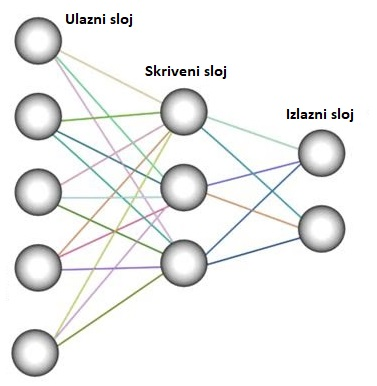
\includegraphics[scale=1]{neural_network_layers.jpeg}
\end{center}
\caption{Višeslojna neuronska mreža sa jednim skrivenim slojem}
\label{fig:neural_network_layers}
\end{figure}


\subsection{Razlog uvodjenja konvolutivnih neuronskih mreža}

Jednostavni zadaci prepoznavanja mogu se dosta dobro rešiti skupovima podataka malih veličina, npr. desetine hiljada slika. Međutim, objekti u realističnim postavkama pokazuju značajnu raznovrsnost, stoga, da bi bilo moguće naučiti prepoznati ih, potrebno je koristiti mnogo veće skupove za treniranje. Da bi se naučilo o hiljadama objekata iz miliona slika, potreban je model sa velikim kapacitetom učenja. Konvolutivne neuronske mreže, koje su detaljno obrađene u ostatku rada, čine jednu takvu klasu modela. One daju jake i uglavnom ispravne pretpostavke o prirodi slika, a njihov kapacitet se moze kontrolisati variranjem njihove dubine i širine. Tako, u poređenju sa standardnim neuronskim mrežama (\textit{mrežama sa propagacijom unapred (eng.} feedforward neural network\textit{)}) sa slojevima sličnih veličina, CNN imaju mnogo manje veza i parametara, tako da ih je lakše trenirati, dok je njihov teoretski najbolji učinak samo nešto lošiji.


\section{Konvolutivne neuronske mreže}	
\label{sec:cnn}

Konvolutivne neuronske mreže predstavljaju podklasu neuronskih mreža koja ima najmanje jedan konvolutivni sloj (a može ih imati i više). Ova vrsta neuronskih mreža je inspirisana vizuelnim korteksom. Svaki put kada osoba nešto vidi, aktivira se niz slojeva neurona, i svaki sloj otkriva skup karakteristika kao što su linije, ivice itd. Viši nivoi slojeva otkritivaju složenije karakteristike kako bi prepoznali ono što je osoba videla. Konvolutivne mreže rade po istom principu i praktično su uvek \textit{duboke neuronske mreže (eng.} deep neural network\textit{)}\footnote{Duboke neuronske mreže su neuronske mreže koje se sastoje od više skrivenih slojeva između ulaznih i izlaznih slojeva (koji na izlazu predviđaju ciljnu promenljivu), koje mogu modelovati i kompleksne nelinearne veze.}, upravo zbog toga što je potrebno od sitnijih detalja, poput uspravnih, kosih i horizontalnih linija, koji obično bivaju detektovani u nižim slojevima mreže, konstruisati složenije oblike poput delova lica. Konvolutivne neuronske mreže se koriste u obradi signala (slike, zvuka), ali i teksta. U odnosu na ostale vrste neuronskih mreža, ističu se u prikupljanju lokalnih informacija (npr. o susednim pikselima na slici ili \textit{,,okružujućim" (eng.} surrounding\textit{)} rečima u tekstu) i smanjenju složenosti modela (brže treniranje, potrebno je manje uzoraka, manja šansa da dodje do \textit{preprilagodjavanja (eng.} overfitting\textit{)}). Konvulativne neuronske mreže se zasnivaju na sposobnosti mreža da iz sirovog signala konstruišu atribute. Nazivaju se konvolutivnim zato što uče \textbf{filtere} (pojam objašnjen u tabeli \ref{tabela_parametri}), čijom konvolutivnom primenom detektuju određena svojstva signala.

Postoji nekoliko različitih arhitektura u polju konvolutivnih neuronskih mreža. One se razlikuju po tipu, broju i rasporedu slojeva, i uglavnom predstavljaju bolju verziju neke od prethodnih mreža (o ovome više reči u poglavlju \ref{struktura_cnn}). Takođe, ono što treba istaći jeste podešavanje parametara mreže. Iako nije moguće izračunati u kom slučaju koji parametar treba imati koju vrednost, u narednom poglavlju (\ref{parametri_sec}) su opisani neki od bitnijih parametara koje svakako treba podesiti pri učenju mreže.


\subsection{Parametri}
\label{parametri_sec}

U ovoj sekciji je dat tabelarni prikaz parametara koji su najznačajniji za implementaciju konvolutivne mreže. U tabeli \ref{tabela_parametri} je dat samo kratak opis svakog od njih radi boljeg razumevanja teksta koji sledi. Ipak, u nastavku je svaki detaljnije opisan.

\begin{table}[h!]
\begin{center}
\caption{Parametri konvolutivne neuronske mreže}
\begin{tabular}{|l|p{60mm}|}
\hline
\textit{Filter/jezgro (eng.} filter/kernel\textit{)} &
- matrica sa težinama za konvoluciju ulaza \newline
- daje meru koliko deo ulaza liči na karakteristiku \newline
- tezine u matricama filtera su izvedene za vreme treniranja podataka
\\
\hline
\textit{Proširenje (eng.} Padding\textit{)} &
- koristi se za dodavanje kolona i redova nula (ili drugih vrednosti) da bi se održala konstantna veličina matrice (mape) nakon konvolucije \newline
- ovaj parametar može da unapredi performanse tako što zadržava informacije u okvirima (tim proširenjima koje dodaje)
\\
\hline 
\textit{Korak (eng.} Stride\textit{)} &
- broj piksela koji se preskače dok se ulaz prelazi vodoravno i uspravno tokom konvolucije, nakon množenja svakog elementa iz ulazne matrice težina s onima u filtru
\\
\hline 
\textit{Broj kanala (eng.} Number of Channels\textit{)} &
- u početku je jednak broju \textit{kanala boja (eng.} color channels\textit{)} ulaza, a u kasnijim stadijumima postaje jednak broju filtera koji su korišćeni za operaciju konvolucije \newline
- što je veći broj kanala, veći je i broj korišćenih filtera, a time je naučeno više karakteristika, pa postoji šansa da dođe do prilagođavanja (i obrnuto)
\\
\hline 
Parametri sloja agregacije &
- ima iste parametre kao i konvolutivni sloj \newline
- uglavnom se koristi \textit{Max-Pooling} opcija (poglavlje \ref{sloj_agregacije}) \newline
- smanjuje dimenzionalnost ulazne reprezentacije (slike, izlazne matrice skrivenog sloja, itd.) tako što čuva maksimalnu vrednost podregiona
\\
\hline 
\end{tabular}
\label{tabela_parametri}
\end{center}
\end{table}


\subsection{Konvolucija slika preko CNN}

%\ref{sec:ime_necega}.

Da bi izvršile klasifikaciju slika, konvolutivne neuronske mreže (preciznije, konvolutivni sloj, detaljnije u poglavlju \ref{konvolucija}) obavljaju neku vrstu pretrage. Ovo se može zamisliti kao mali pokretni (ili klizni) prozor (prikazano na slici \ref{fig:filter_movement01}) koji klizi s leva na desno preko veće slike, i nastavlja s leve strane kada dođe do kraja jednog prelaza (kao kod pisaće mašine). Taj pokretni prozor - koji ustvari predstavlja filter, može da prepozna samo jednu stvar, recimo kratku vertikalnu liniju (tri tamna piksela naslagana jedan na drugi). Slično, neki drugi filter može da služi za prepoznavanje horizontalnih linija, i on se takođe pomera preko piksela slike, tražeći podudaranja. Rezultat koji se postiže filterima koji prepoznaju vertikalne i horizontalne linijije prikazan je na slici \ref{fig:edges}.

% TODO: Slike se ne prikazuju u .pdf fajlu tamo gde su pozicionirane u .tex fajlu, iako je navedeno [h!]

\begin{figure}[h!]
\begin{center}
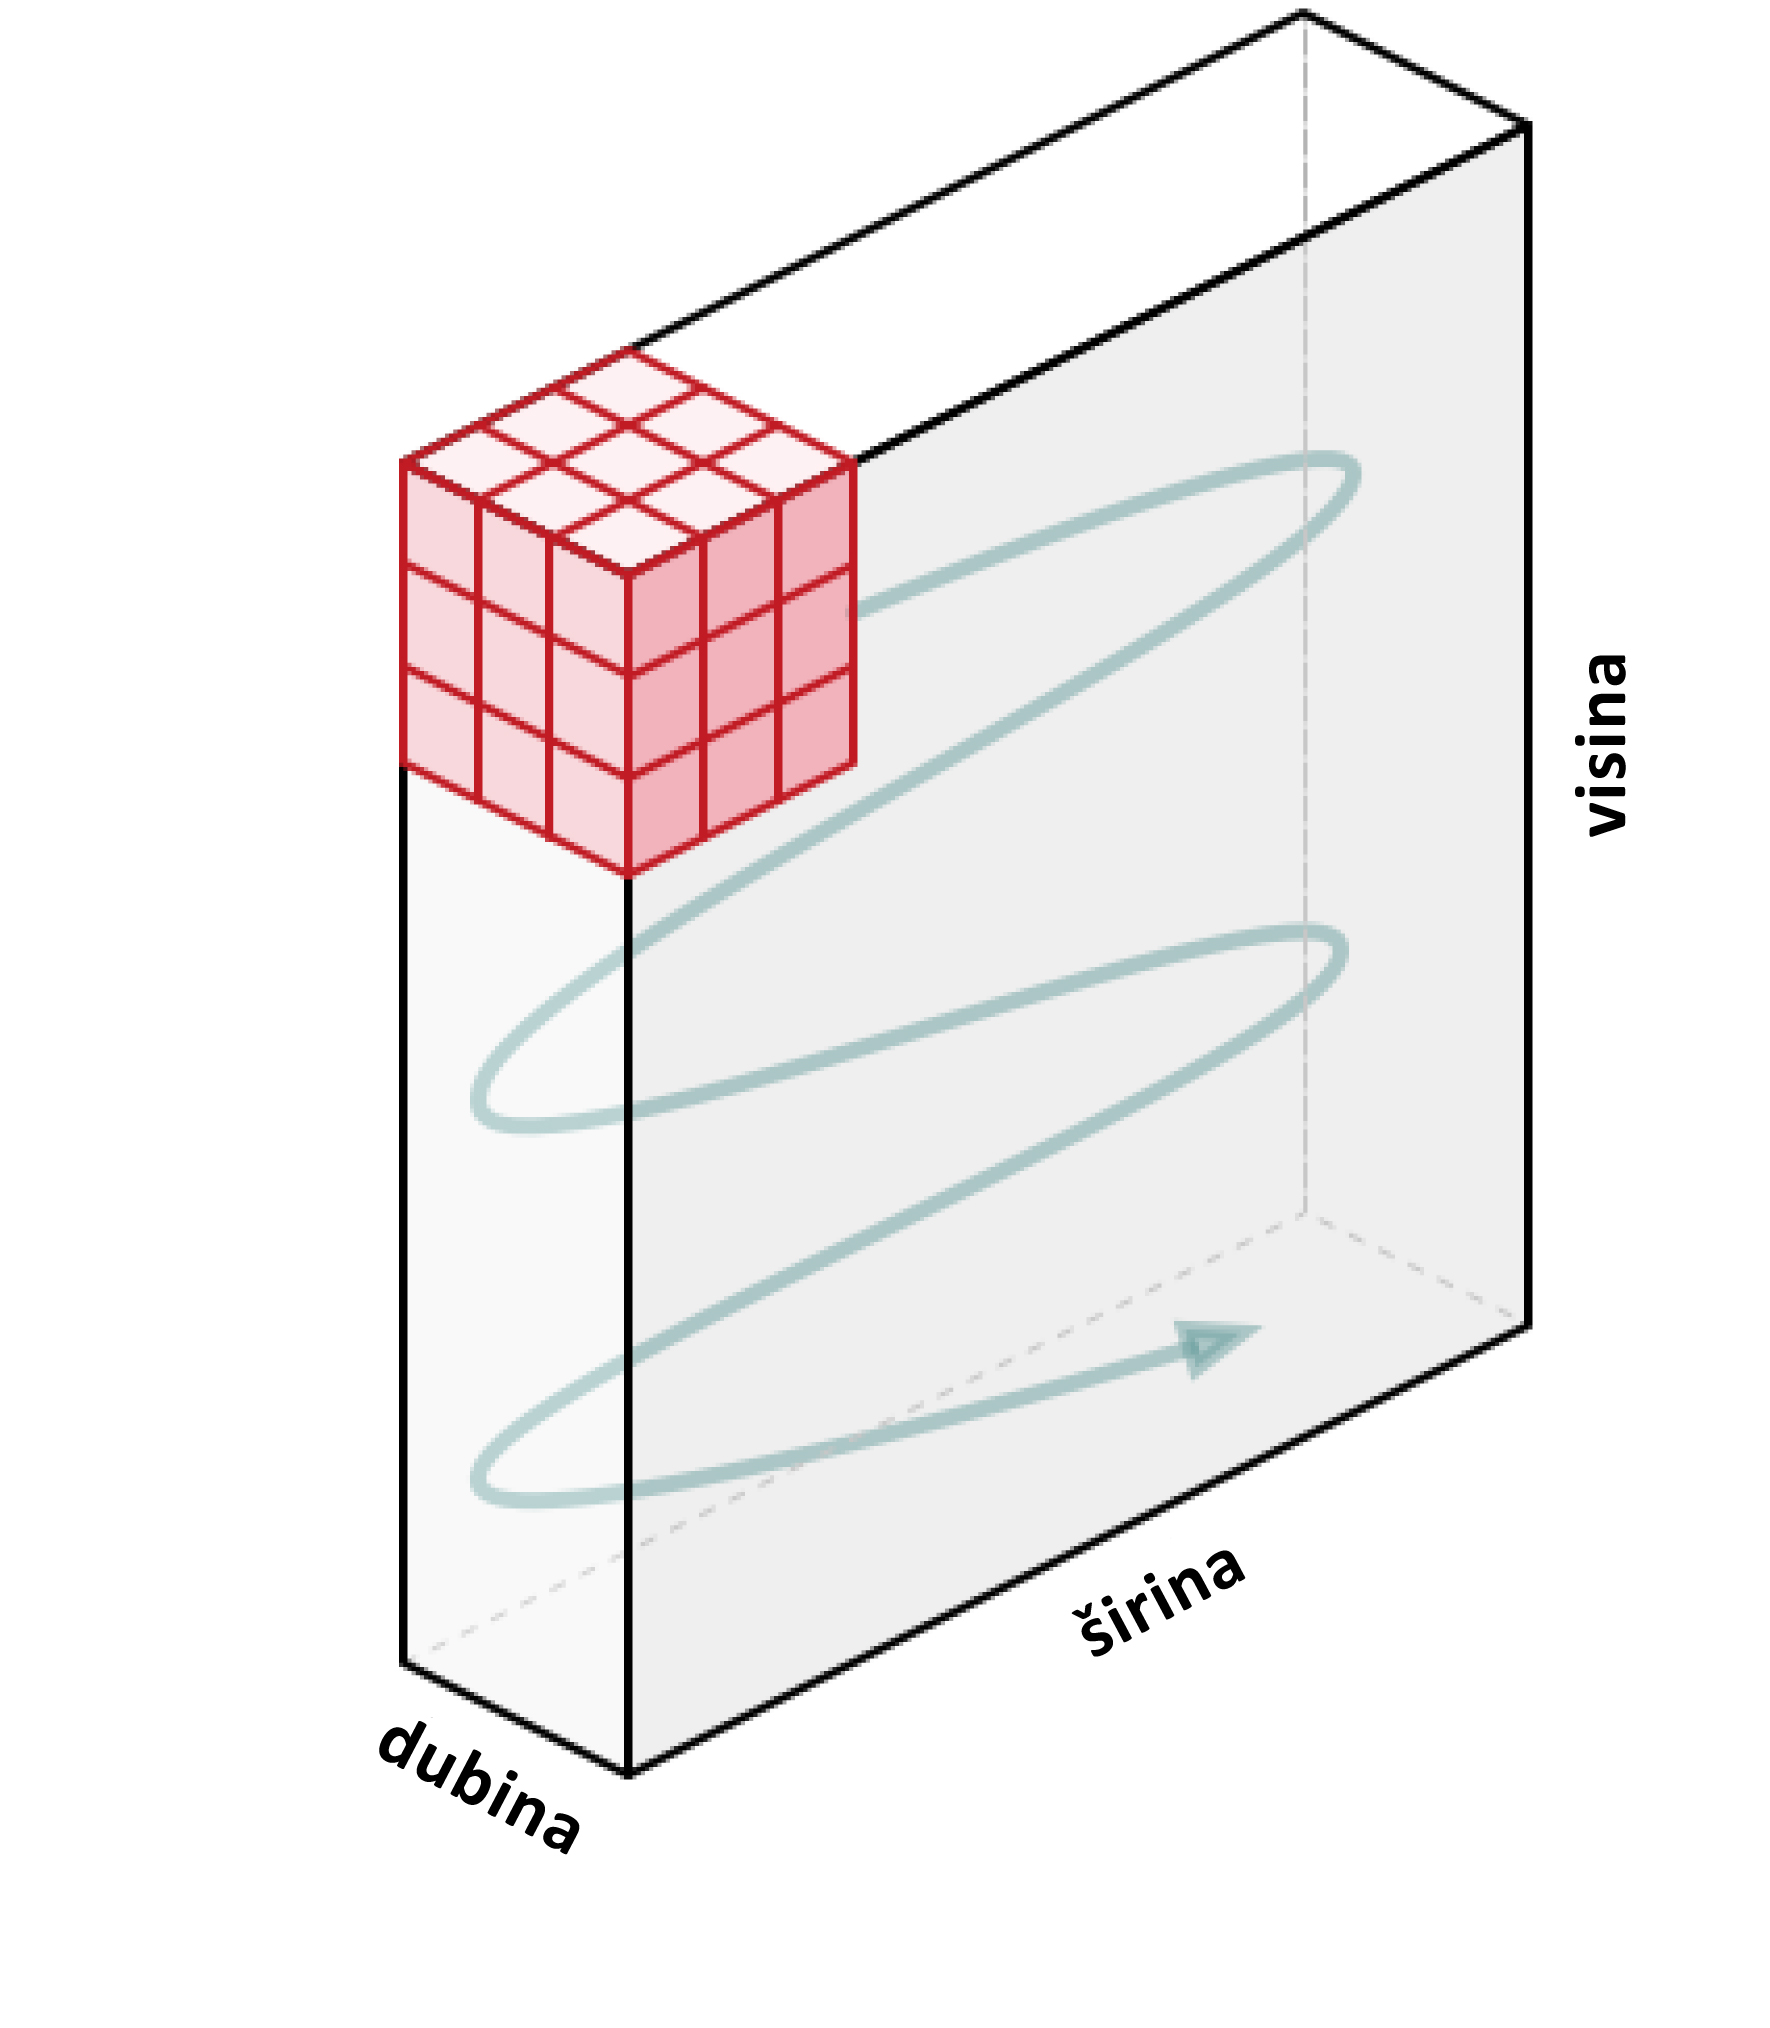
\includegraphics[scale=0.4]{filter_movement01.jpg}
\end{center}
\caption{Kretanje filtera}
\label{fig:filter_movement01}
\end{figure}


\begin{figure}[h!]
\begin{center}
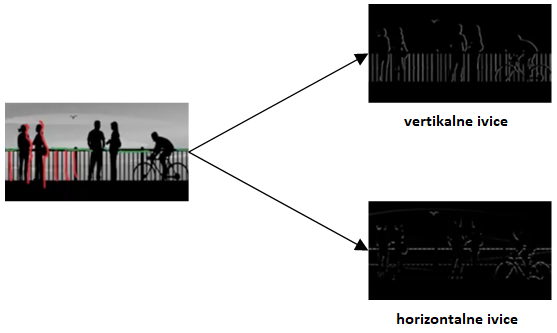
\includegraphics[scale=1]{edges.png}
\end{center}
\caption{Detektovanje vertikalnih i horizontalnih ivica}
\label{fig:edges}
\end{figure}

Svaki put kada dođe do poklapanja (filtera sa ulazom), ono se mapira u prostor sa karakteristikama - koji se zove \textit{\textbf{mapa karakteristika} (eng.} feature maps\textit{)}, koji je specifican za taj vizuelni element. U tom prostoru (tj. mapi) se čuva (odnosno beleži) lokacija svakog poklapanja sa vertikalnom linijom. Konvolutivna mreža pokreće mnogo pretraga nad jednom istom slikom. Na početnom sloju mreže koriste se filteri koji prepoznaju horizontalnu liniju, vertikalnu liniju i dijagonalnu liniju, da bi kreirali mapu ivica slike. U narednim koracima (odnosno slojevima) posmatraju se kombinacije ovih ivica i tako prepoznaju složeniji oblici. Ovo je demonstrirano na slici \ref{fig:learning}. U narednim poglavljima je objašnjeno iz čega se  konvolutivne neuronske mreže sastoje i kako ti gradivni elementi zapravo funkcionišu.

\begin{figure}[h!]
\begin{center}
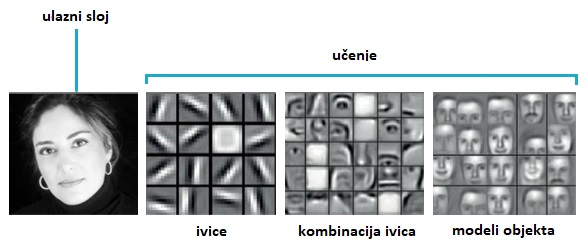
\includegraphics[scale=0.9]{learning.jpg}
\end{center}
\caption{Učenje mreže}
\label{fig:learning}
\end{figure}


\subsection{Unutrašnja struktura CNN}
\label{struktura_cnn}
Unutrašnja struktura konvolutivne mreže se sastoji od nekoliko naizmeničnih \textit{\textbf{konvolutivnih slojeva} (eng.} convolution layer\textit{)} i \textit{\textbf{slojeva agregacije} (eng.} pooling layer\textit{)}, pri čemu je dozvoljeno pojavljivanje iste vrste sloja više puta (prikazano na slici \ref{fig:cnn_layers}). Nakon uzastopnog smenjivanja ova dva sloja sledi \textit{\textbf{potpuno povezani sloj} (eng.} fully connected layer\textit{)}, koji se takođe može ponavljati više puta. Izlazi konvolutivnog sloja su dvodimenzionalni i nazivaju se mapama karakteristika. Oni se transformisu nelinearnom \textbf{aktivacionom funkcijom}. U konvolutivnim mrežama kao aktivacione funkcije najčešće se koriste \textit{\textbf{prečišćena linearna jedinica} (eng.} Rectified Linear Unit, ReLu\textit{)}\footnote{ReLu funkcija se definiše kao: f(x) = max(0,x). Prednost ReLu nad sigmnoidnom funkcijom (koja se takođe može koristiti kao aktivaciona funkcija) je što treniranje obavlja mnogo brže.} (na izlazu iz konvolutivnog sloja) i \textit{\textbf{softmaks klasifikator} (eng.} softmax classifier\textit{)} (na izlazu iz poslednjeg, potpuno povezanog, sloja mreže). U nastavku rada je svaki od tri sloja obrađen pojedinačno u poglavljima \ref{konvolucija}, \ref{sloj_agregacije}, \ref{potpuno_povezani_sloj}, dok se o aktivacionim funkcijama detaljnije govori u poglavlju \ref{aktivaciona_funkcija}.


\begin{figure}[h!]
\begin{center}
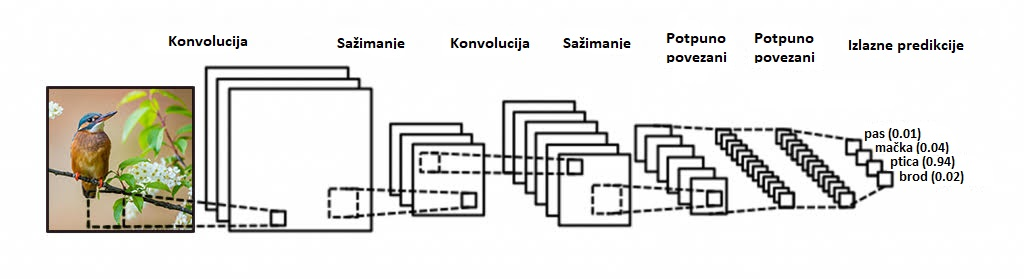
\includegraphics[scale=0.62]{cnn_layers.jpg}
\end{center}
\caption{Arhitektura konvolutivne neuronske mreže}
\label{fig:cnn_layers}
\end{figure}

Kako su moguće različite kombinacije različitih slojeva, prirodno je da postoji više arhitektura konvolutivnih neuronskih mreža. Svaka od tih arhitektura ima svoje prednosti i mane, i u zavisnosti od problema drugačija arhitektura daje bolje (odnosno gore) rezultate. U sledećoj listi su nabrojane i ukratko opisane samo neke od najpoznatijih arhitektura konvolutivnih neuronskih mreža:

\begin{itemize}

\item \textbf{LeNet-5} - Ovu arhitekturu je napravio Yann LeCunn krajem 20. veka, a koristila se za čitanje zip kodova, cifara itd. LeNet-5 arhitektura se sastoji iz dva skupa konvolutivnih slojeva i slojeva agregacije, koji su praćeni \textit{poravnavajućim konvolutivnim slojem (eng.} flattening convolutional layer\textit{)}, za kojim slede dva potpuno-povezana sloja, a zatim softmaks klasifikator.

\item \textbf{AlexNet} - Ovo je jedna od prvih dubokih neuronskih mreža. Sastoji se iz pet konvolutivnih slojeva praćena sa tri potpuno povezana sloja. Ovu mrežu je napravio Alex Krizhevsky, koji je koristio prečišćenu linearnu jedinicu - ReLu za ne-linearni deo umesto Tanh ili Sigmoid funkcije, koje su bile standardne za tradicionalne neuronske mreže.

\item \textbf{VGG16} - Ova arhitektura predstavlja unapređenje arhitekture AlexNet. U njoj su veliki filteri (jezgra) zamenjeni sa više malih 3x3 filtera, jedan za drugim\footnote{Više manjih filtera se pokazuje boljim nego jedan veliki filter (jezgro), zato što više ne-linearnih slojeva povećavaju dubinu mreže što im omogućava da uče kompleksnije karakteristike (i to po manjoj ceni).}.

% Objašnjenje: koliko ima filtera, toliko ima izlaznih mapa karakteristika - a to je dubina mreže, što ih je više - to je mreža dublja i može da uči kompleksnije karakteristike.

\item \textbf{GoogLeNet} - Ova arhitektura ima čak 22 sloja. Brža je i manja od Alexnet, ali i mnogo preciznija. Ideja ove mreže jeste da se napravi model koji će moći da se koristi i na \textit{pametnom telefonu (eng.} smart-phone\textit{)}.

\end{itemize}


\subsection{Konvolutivni sloj}
\label{konvolucija}

Konvolutivni sloj je glavni deo konvolutivne neuronske mreže koji radi najviše izračunavanja u mreži. Njegova uloga je konstrukcija novih atributa. To je prvi sloj koji ekstraktuje karakteristike iz ulazne slike. Konvolucija je matematička operacija koja uzima dva ulaza - dve matrice f i g, dimenzija m x n i p x q, a definisana je na sledeći način:
$$(f * g)_{ij} = \sum_{k=0}^{p-1} \sum_{l=0}^{q-1} f_{i-k, i-l}g_{k, l}$$
Matrica f predstavlja ulaz, poput slike, a matrica g filter. Određena ulazna reprezentacija podatka (originalna slika) konvolvira se sa filterom sa određenim parametrima (ti parametri predstavljaju i parametre konvolutivne neuronske mreže). Procesom učenja ovi parametri (težine koje je potrebno naučiti kako bi mreža davala dobre rezultate) se podešavaju i bivaju naučeni. Filteri su najcešce manjih prostornih dimenzija od ulaza, ali uvek su jednake dubine kao i ulaz. Kao što je vec rečeno, konvolucijska jezgra (filteri) filtriraju sliku, tj. mapu karakteristika kako bi dobili neku korisnu informaciju kao što je recimo određeni oblik, boja ili ivica.

Tokom prvog prolaza svaki filter se pomera po širini i visini ulaza i računa se skalarni proizvod ulaza i vrednosti filtera (prikazano u formuli iznad). Ako obe matrice imaju visoke vrednosti na istim pozicijama, onda će i vrednost skalarnog proizvoda biti velika. A, ako nemaju, onda će i vrednost skalarnog proizvoda biti mala. Na taj način, samo na osnovu te vrednosti, može se zaključiti da li sadržaj slike odgovara sadržaju koji filter traži.

Izlaz jednog filtera je dvodimenzioni niz. Ako postoji više filtera, izlaz iz konvolutivnog sloja su rezultati svih filtera (mape karakteristika) poredjani po dubini. Broj mapa karakteristika na izlazu, odnosno broj primenjenih filtera, predstavlja \textbf{dubinu mreže}. Operacijom konvolucije dobija se transformirana slika dimenzije I*K, gde je I dimenzija ulazne matrice slike, a K dimenzija filtera koji je primenjen nad tom slikom. Takođe, dobijena transformacija je lokalna tj. pikseli izlaza zavise od lokalnih, susednih piksela ulaza. Ceo proces konvolucije, za koji je upotrebljen filter dimenzije 3x3 i ulazna matrica dimenzije 8x8, prikazan je na slici \ref{fig:convolution}. U podpoglavljima \ref{prosirivanje} i \ref{aktivaciona_funkcija} su opisani parametri koji bitno utiču na ishod rada mreže.

% TODO: Naći operator x - ne radi \times ni \wedge!

% TODO: Malo štrči naslov slike u odnosu na ostatak teksta! Ne može sa \newline ili sa \\ da se prebaci deo teksta u novi red!

\begin{figure}[h!]
\caption{Konvolucija primenom filtera dimenzije 3x3 na matricu dimenzije 8x8}
\centering
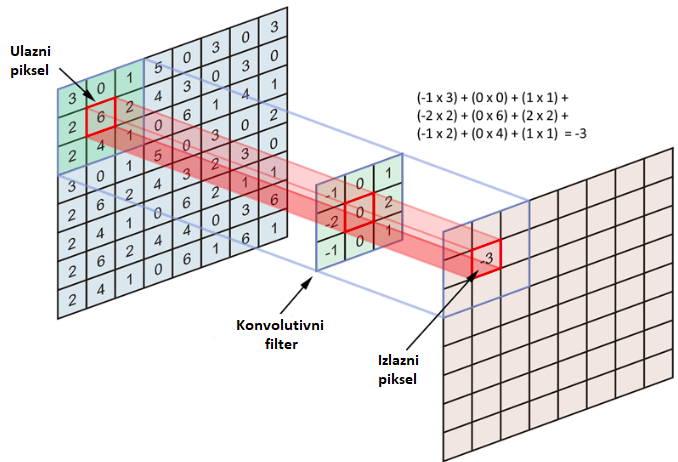
\includegraphics[scale=0.9]{convolution.png}
\label{fig:convolution}
\end{figure}

\subsubsection{Proširivanje}
\label{prosirivanje}

Formula konvolucije koja je data u poglavlju \ref{konvolucija} nije definisana za sve indekse i = $\overline{0, m-1}$ i j = $\overline{0, n-1}$. Na primer, ako je i, j = 0 i k, l $>$ 0, vrednost $f_{i-k, i-l}$ nije definisana. Ukoliko bi se u obzir uzele samo definisane vrednosti, dimenzija konvolucije bi bila manja od dimenzije matrice f. Međutim, to nije uvek poželjno, i može se izbeći tako što se vrši \textbf{proširivanje} matrice f, na primer nulama ili vrednostima koje su već na obodu, tako da veličina rezultujuće matrice bude jednaka veličini matrice f pre proširivanja. Ovo je prikazano na slici \ref{fig:padding}. Takođe, prilikom računanja konvolucije, filter se duž slike ne mora pomerati za jedan piksel, već za neki veći \textbf{korak} (pojam opisan u tabeli \ref{tabela_parametri}).

\begin{figure}[h!]
\begin{center}
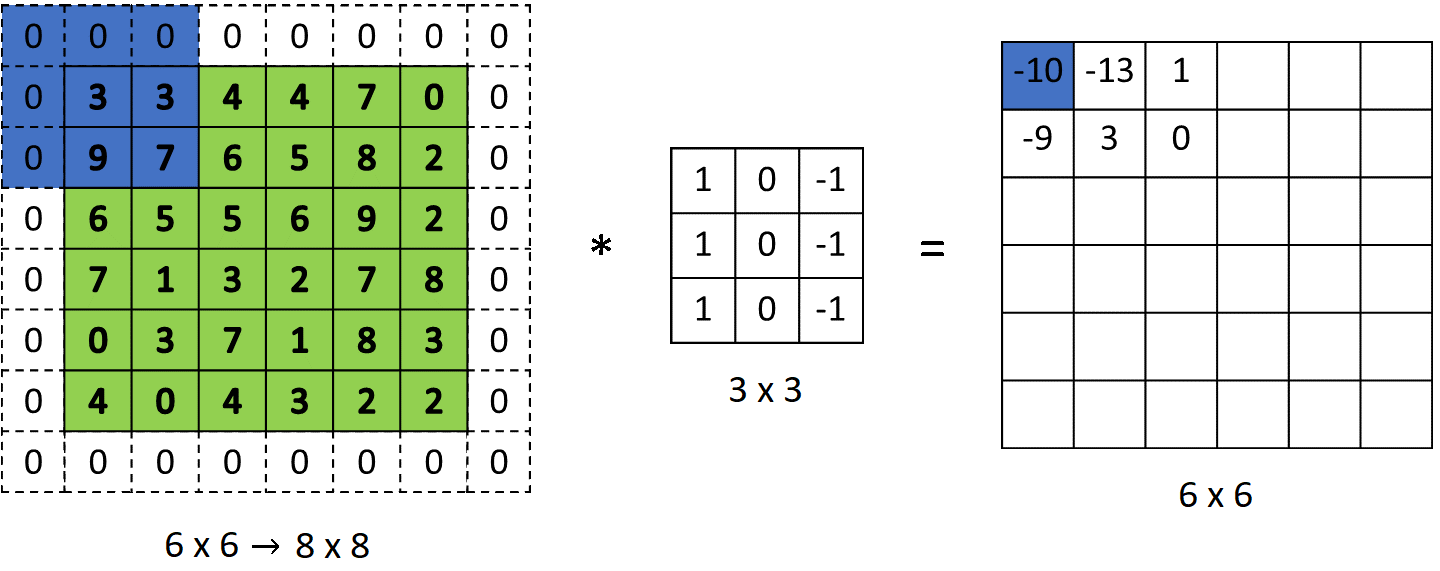
\includegraphics[scale=0.38]{padding.png}
\end{center}
\caption{Primer proširivanja ulazne matrice nulama}
\label{fig:padding}
\end{figure}


\subsubsection{Aktivaciona funkcija}
\label{aktivaciona_funkcija}

U konvolutivnim slojevima kao aktivaciona funkcija se najčešće koristi ReLu (Rectified Linear Unit) funkcija. Definisana je kao $$ f(z) = max(0, z). $$ To znači da će negativne piksele mape karakteristika nastale konvolucijom da postavi na nulu i neće aktivirati odgovarajuće neurone. A pozitivne piksele neće menjati. Na taj način, ReLu ne aktivira sve neurone u istom trenutku, čime ubrzava rad mreže i čini je efikasnijom. Na slici \ref{fig:relu_fja} se može videti kako ReLU funkcija izgleda, a na slici \ref{fig:relu_transform} kako se pomoću nje transformiše mapa karakteristika.

\begin{figure}[h!]
\begin{center}
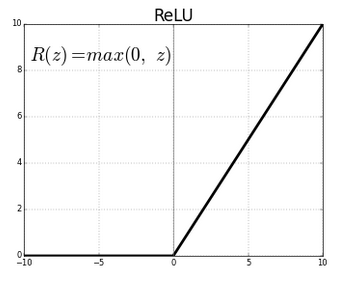
\includegraphics[scale=0.38]{relu2.png}
\end{center}
\caption{Izgled ReLU funkcije}
\label{fig:relu_fja}
\end{figure}


\begin{figure}[h!]
\begin{center}
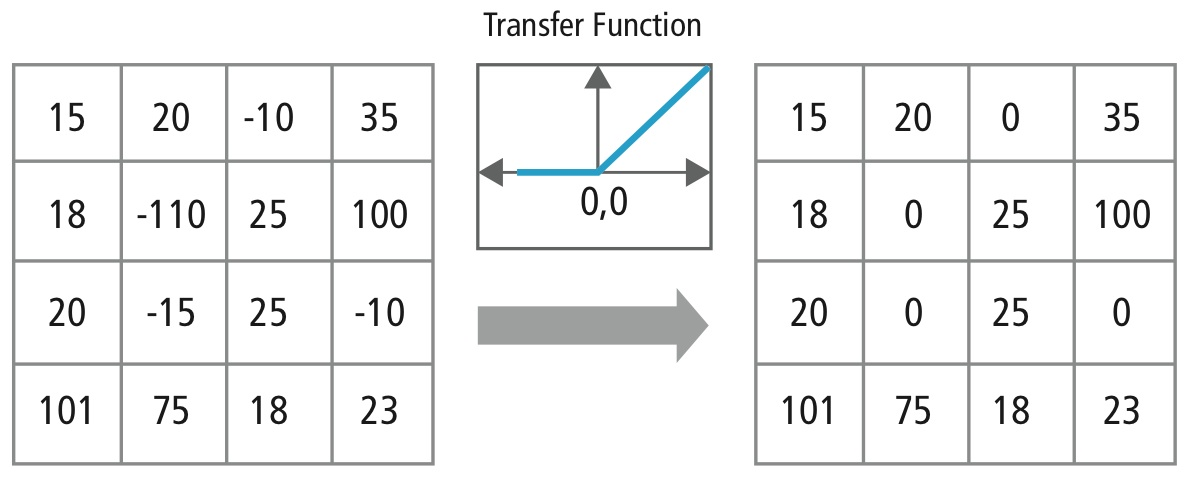
\includegraphics[scale=0.20]{relu1.jpg}
\end{center}
\caption{Primer rada ReLU funkcije nad mapom karakteristika}
\label{fig:relu_transform}
\end{figure}

\newpage


\subsection{Sloj agregacije}
\label{sloj_agregacije}

Uloga sloja za agregaciju je smanjenje broja parametara kada su slike prevelike, kao i smanjenje broja operacija u višim slojevima mreže. Agregacija smanjuje dimenzionalnost svake mape, ali zadržava važne informacije. Sve to rezultuje smanjenjem računske zahtevnosti pri optimizaciji i pomaže u kontroli \textit{overfitinga}. Zato je poželjno da slojevi za agregaciju prate konvolutivne slojeve kako bi postepeno smanjili prostornu veličinu (širinu i visinu) prikaza podataka.

Često konačni zadatak postavlja neko globalno pitanje o slici, na primer, da li sadrži mačku? Stoga, čvorovi zadnjeg sloja moraju biti osetljivi na celi ulaz. Postepenom agregacijom informacija, stvarajući sve grublje i grublje mape karakteristika, postiže se taj cilj da se na kraju nauči globalna reprezentacija, zadržavajući sve prednosti konvolutivnih slojeva na srednjim slojevima obrade.

Sloj agregacije ukrupnjuje informacije, tako sto računa neku jednostavnu funkciju agregacije susednih jedinica prethodnog sloja, poput \textit{maksimuma (eng.} Max pooling\textit{)}, koji vraća maksimalnu vrednost dela slike pokrivene filterom, ili \textit{proseka (eng.} Average pooling\textit{)}, koji vraća prosečnu vrednost dela slike pokrivene filterom. Funkcija koja vraća prosečnu vrednost se u praksi toliko ne koristi, već se javlja iz istorijskih razloga, dok se funkcija koja računa maksimalnu vrednost mnogo bolje pokazala u praksi, te se ona skoro uvek koristi. Ukoliko agregira, na primer, 3 x 3 piskela, onda je broj izlaza ovog sloja 9 puta manji od broja izlaza prethodnog. Kada se računa maksimum, dolazi do zanemarivanja informacija o tome gde je precizno neko svojstvo (poput uspravne linije) pronađeno, ali se ne gubi informacija da je ono pronađeno. Ovakva vrsta zanemarivanja informacije često ne šteti cilju koji treba postići. Na primer, ako su na slici pronađeni kljun i krila, informacija o tačnoj poziciji najverovatnije nije bitna za odlučivanje da li se na slici nalazi ptica. Ipak, ukoliko je potrebno napraviti mrežu koja igra igru u kojoj su pozicije objekata na ekranu bitne, nije poželjno koristiti agregaciju. Slede dva ilustrovana primera, a onda poglavlje o sloju koji se nadovezuje na agregacioni (poglavlje \ref{potpuno_povezani_sloj}).

Na slici \ref{fig:pool} je prikazana operacija agregacije primenjena na ulaz dimenzija 224x224x64, uz pomoć filtera veličine 2 i koraka veličine 2. Izlaz koji se dobija je dimenzija 112x112x64. Može se primetiti da je dubina matrice ostala očuvana. Naime, agregirajući sloj redukuje veličinu posebno, tj. nezavisno za svaki \textit{sloj dubine (eng.} depth slice\textit{)} ulazne veličine.

\begin{figure}[h!]
\begin{center}
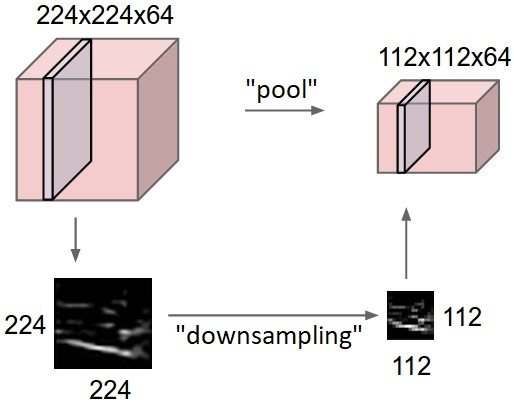
\includegraphics[scale=0.4]{pool.jpeg}
\end{center}
\caption{Pool}
\label{fig:pool}
\end{figure}

Na slici \ref{fig:maxpool} je prikazan izlaz koji se dobija kada se na ulaznu matricu dimenzije 4x4 primeni Maxpool metod uz pomoć filtera dimenzije 2x2 i koraka 2. Naime, u ovom primeru se računa maksimalna vrednost nad svakim blokom od četiri broja.
 
\begin{figure}[h!]
\begin{center}
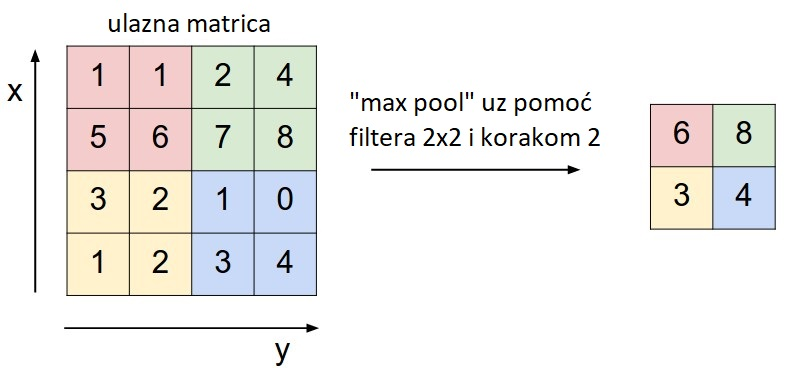
\includegraphics[scale=0.4]{maxpool.jpeg}
\end{center}
\caption{Maxpool}
\label{fig:maxpool}
\end{figure}


\subsection{Potpuno povezani sloj}
\label{potpuno_povezani_sloj}

Nakon što su u konvolutivnom i agregativnom sloju sakupljene informacije o slici, sledeće što je potrebno uraditi jeste zaključiti kojoj klasi pripada ta slika. Za to se koristi jedan ili više potpuno povezanih slojeva (eng. \textit{fully connected layer} ili \textit{dense layer}). 

U potpuno povezanom sloju, svaki neuron je povezan sa svakim neuronom iz prethodnog sloja, kao što je to slučaj kod običnih neuronskih mreža. Taj sloj kao ulaz očekuje vektor, što znači da je prvo potrebno ispraviti (eng. \textit{flatten}) mapu karakteristika, dobijenu nakon konvolucije i agregacije, u vektor. U svim slojevima, osim u poslednjem, može da se koristi ReLU aktivaciona funkcija.

Poslednji potpuno povezani sloj treba da ima onoliko neurona koliko ima i klasa, kako bi mogao da odredi koju klasu da pridruži slici. U ovom sloju je najbolje koristiti softmax aktivacionu funkciju. Softmax funkcija određuje verovatnoću pripadnosti slike svakoj od klasa. Nakon njene primene, dobija se vektor vrednosti koje odgovaraju verovatnoćama i koje u zbiru daju vrednost 1. Zahvaljujući njoj, slika se klasifikuje u onu klasu kojoj odgovara najveća verovatnoća pripadnosti. Softmax funkcija je definisana kao: $$ S(z_i) = \frac{e^z_i}{\sum_{j=1}^{K}e^z_j},  i = 1,...,K,  z = (z_1,...,z_K) $$ gde je z ulazni vektor od K realnih brojeva. 

U sloju koji koristi softmax aktivacionu funkciju, obično se za funkciju određivanja greške klasifikacije uzima \textit{categorical crossentropy}. Ona se koristi ukoliko su podaci takvi da jedna instanca tih podataka može da pripada samo jednoj klasi. \textit{Categorical crossentropy} upoređuje raspodelu verovatnoća predviđenih klasa sa raspodelom koja odgovara pravim klasama. Ova funkcija je definisana kao:
$$ H(y, \hat{y}) = -\sum_{i} y_i\cdot log(\hat{y})) $$ gde \textit{y} predstavlja vektor pravih raspodela, a $\hat{y}$ vektor predviđenih raspodela.

\section{Implementacija i eksperimentalni rezultati}
\label{sec:implementacija_i_eksperimentalni_rezultati}


Neuronsku mrežu smo implementirale u programskom jeziku Python korišćenjem Keras biblioteke. Kao podatke za trening i testiranje, koristile smo slike iz baze podataka kineskih saobraćajnih znakova \cite{CTSD}. Baza sadrži 6164 slika saobraćajnih znakova podeljenih u 58 klasa, pri čemu trening skup sadrži 4170, a test skup 1994 slike. Međutim, nisu sve klase imale podjednak broj slika. Za neke je postojalo 5 slika na kojima bi mreza mogla da trenira, a za neke oko 400. Takođe, zbog prevelike količine podataka, izvršavanje programa je bilo mnogo sporo. Zbog svega toga, odlučile smo da koristimo samo jedan deo te baze i izdvojile 10 klasa koje su imale približno jednak broj slika. Nakon toga, dobile smo trening skup od 1693 slika i test skup od 764 slike. Na slici \ref{fig:trening_skup} je prikazan po jedan znak iz svake klase trening skupa, zajedno sa brojem elemenata te klase. Slično, ti podaci o test skupu, mogu se videti na slici \ref{fig:test_skup}.

\begin{figure}[h!]
\begin{center}
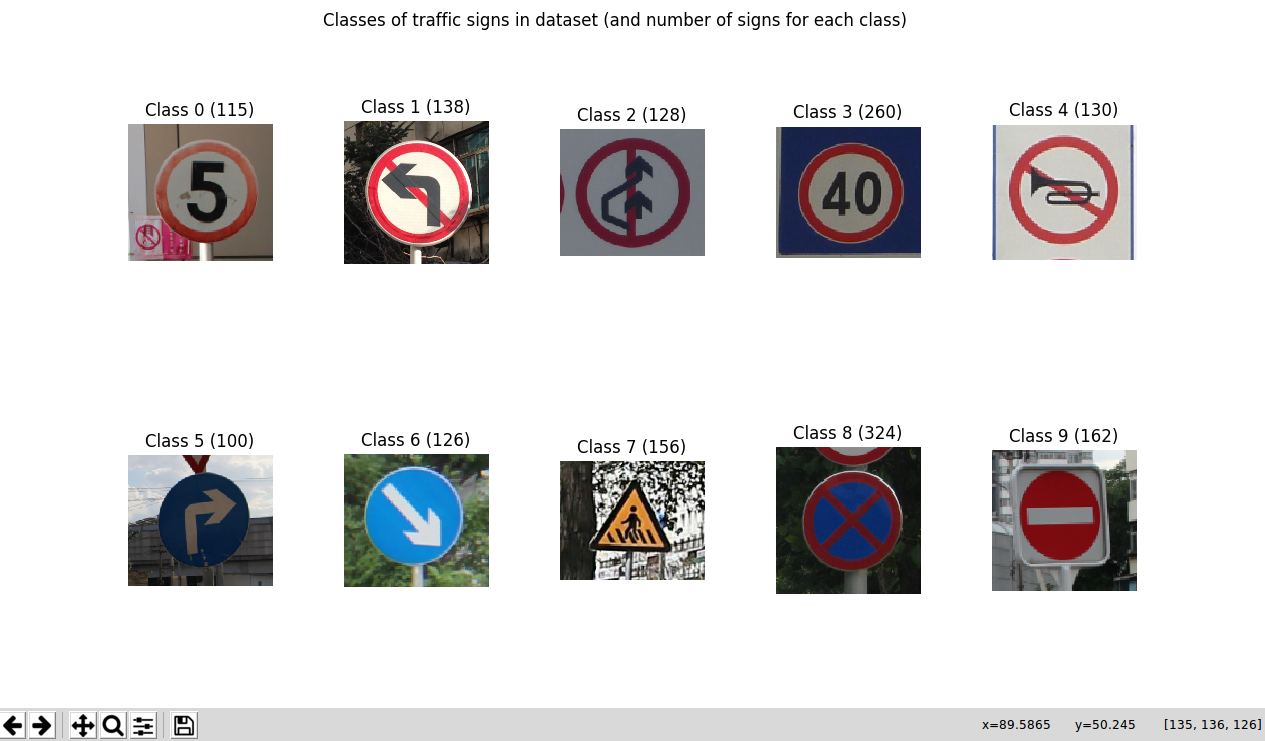
\includegraphics[scale=0.25]{trening_skup.png}
\end{center}
\caption{Trening skup}
\label{fig:trening_skup}
\end{figure}

\begin{figure}[h!]
\begin{center}
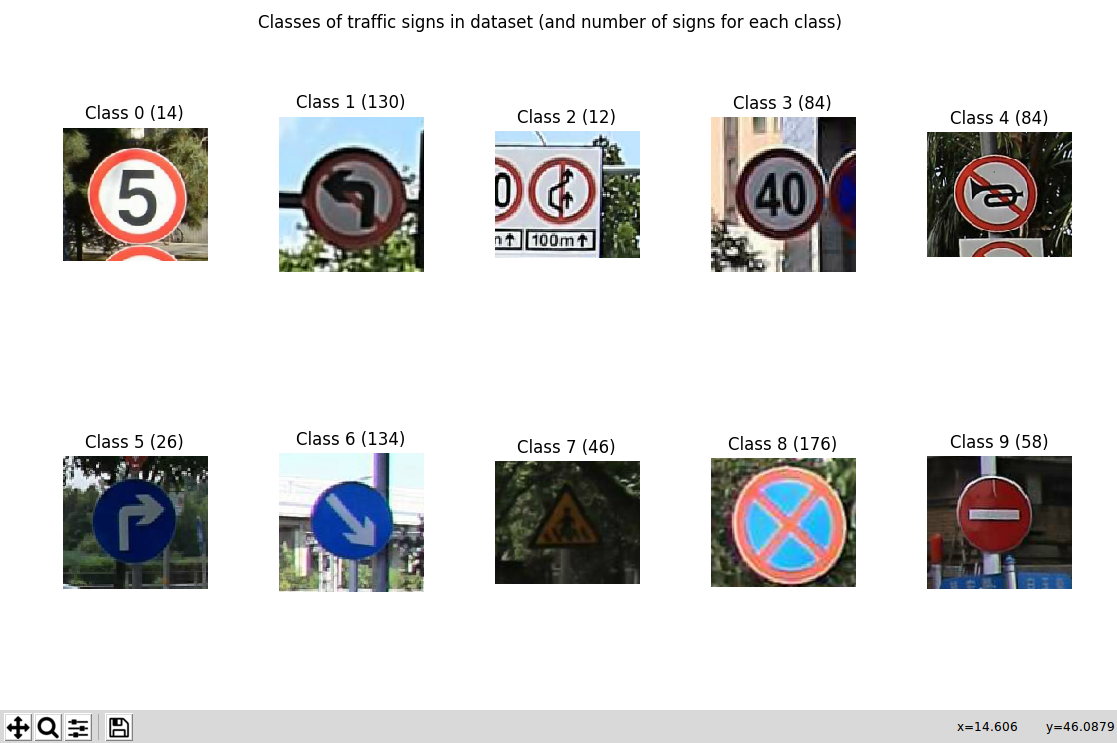
\includegraphics[scale=0.25]{test_skup.png}
\end{center}
\caption{Test skup}
\label{fig:test_skup}
\end{figure}

U narednim poglavljima će biti predstavljeni neki od modela konvolutivnih neuronskih mreža koje smo pravile, a koje su davale najbolje rezultate.

\subsection{Model 1}
\label{sec:model_1}

Jedan od prvih modela koji je imao veći uspeh na test podacima prikazan je u kodu \ref{code:model1}. Sastoji se iz četiri konvolutivna, dva agregativna i dva potpuno povezana sloja. Detaljna arhitektura mreže se može videti na slici \ref{fig:model1_arh}. U svim konvolutivnim slojevima veličina jezgra je 3x3, a broj filtera na izlazu iz konvolucije je 32. Takođe, u svakom se koristi ReLU aktivaciona funkcija. U sloju agregacije, sažimanje se vrši biranjem maksimalne vrednosti dela mape karakteristika koji je prekriven filterom. Kako ne bi došlo do preprilagodjavanja modela trening podacima, povremeno je, pomoću funkcije Dropout(), isključivan određen broj nasumično odabranih neurona. Nakon agregacija je isključeno 20\% neurona, a pre poslednjeg, potpuno povezanog, sloja 50\%. Poslednji potpuno povezani sloj ima onoliko neurona koliko ima klasa i koristi softmax aktivacionu funkciju.

Učenje modela je sprovedeno u 30 epoha. Batch size je postavljen na 32, što znači da će u svakoj iteraciji biti uzeta 32 primerka iz trening skupa koja će biti propagirana kroz mrežu. Optimizacija modela je izvršena pomoću gradijentnog spusta. Takođe, pre početka treninga, sve slike su skalirane na istu veličinu, 64x64 piksela.


\begin{lstlisting}[caption={Model 1},frame=single, label=code:model1]
def cnn_model():
    
    model = Sequential()

    model.add(Conv2D(filters = 32, kernel_size = (3, 3), 
    		padding='same', input_shape=(IMG_SIZE, IMG_SIZE, 3), 
    		data_format="channels_last", activation='relu'))
    model.add(Conv2D(filters = 32, kernel_size = (3, 3), 
    		activation='relu'))
    model.add(MaxPooling2D(pool_size=(2, 2)))
    model.add(Dropout(0.2))

    model.add(Conv2D(filters = 32, kernel_size = (3, 3), 
    		padding='same', activation='relu'))
    model.add(Conv2D(filters = 32, kernel_size = (3, 3), 
    		activation='relu'))
    model.add(MaxPooling2D(pool_size=(2, 2)))
    model.add(Dropout(0.2))
    
    model.add(Flatten())
    model.add(Dense(512, activation='relu'))
    model.add(Dropout(0.5))
    model.add(Dense(NUM_OF_CLASSES, activation='softmax'))
    
    model.summary()
    return model


batch_size = 32
epochs = 30
lr = 0.01   #learning rate

model = cnn_model()

# optimizacija pomocu gradijentnog spusta
sgd = SGD(lr=lr, decay=1e-6, momentum=0.9, nesterov=True)

model.compile(loss='categorical_crossentropy', optimizer=sgd, 
			  metrics=['accuracy'])

def lr_schedule(epoch):
    return lr * (0.1 ** int(epoch / 10))

model.fit(images, classes,
          batch_size=batch_size,
          epochs=epochs,
          validation_split=0.2,
          callbacks=[LearningRateScheduler(lr_schedule), 
          			 ModelCheckpoint('model.h5', save_best_only=True)])
\end{lstlisting}


\begin{figure}[h!]
\begin{center}
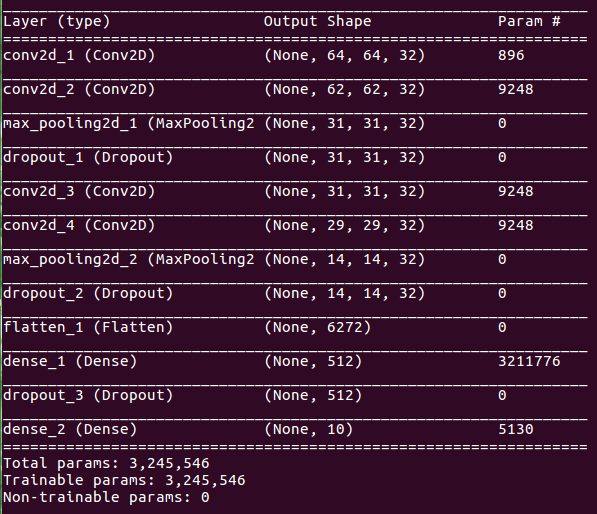
\includegraphics[scale=0.45]{model1_arhitektura.png}
\end{center}
\caption{Slojevi modela neuronske mreže}
\label{fig:model1_arh}
\end{figure}

Na slici \ref{fig:model1_trening_acc} možemo videti da je preciznost modela na trening skupu tokom poslednje tri epohe varirala oko 0.99 i 1.0. Na slici \ref{fig:model1_test_acc} možemo videti kako se model pokazao na test skupu. Preciznost (\textit{accuracy}, tj. broj tačno klasifikovanih instanci / ukupan broj instanci) je jednaka 0.882. Vidimo da je i preciznost (\textit{precision}) koja se odnosi na svaku od klasa dosta visoka (osim za klase 0 i 5)

\begin{figure}[h!]
\begin{center}
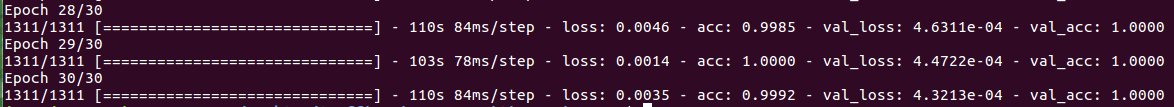
\includegraphics[scale=0.35]{model1_trening_acc.png}
\end{center}
\caption{Preciznost na trening podecima}
\label{fig:model1_trening_acc}
\end{figure}

\begin{figure}[h!]
\begin{center}
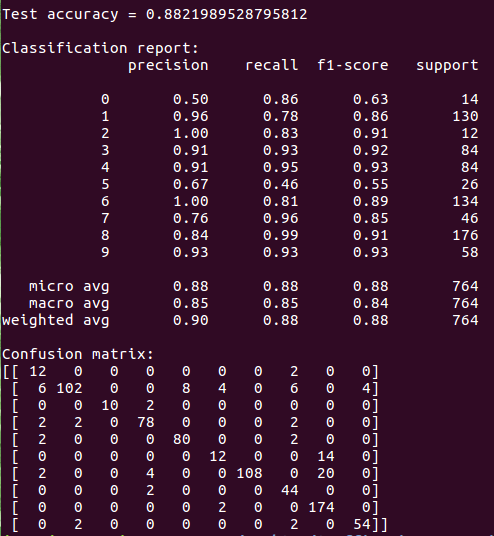
\includegraphics[scale=0.45]{model1_test_acc.png}
\end{center}
\caption{Preciznost na test podecima}
\label{fig:model1_test_acc}
\end{figure}

\newpage

\subsection{Model 2:  LeNet-5}
\label{sec:model_2}


Još bolje rezultate smo dobile pomoću LeNet-5 mreže \cite{leNet}. LeNet-5 mrežu je 1990ih napravio Yann LeCunn. Mreža se sastoji iz 7 slojeva, pri čemu se ne računa ulazni sloj. Sve slike smo skalirale na večičinu 32x32 piksela, jer ova mreža kao ulaz očekuje slike tih dimenzija. Prvi konvolutivni sloj na izlazu daje 6 mapa karakteristika, koristi jezgro veličine 3x3 i kao aktivacionu funkciju koristi ReLU. Nakon njega sledi sloj agregacije u kom se sažimanje vrši biranjem prosečne vrednosti dela mape karakteristika koji je prekriven filterom. 
Još jednom se ponavljaju ova dva sloja, s tim što sada konvolutivni sloj vraća 16 mapa karakteristika. Nakon ispravljanja mape karakteristika u vektor, taj vektor se prosleđuje potpuno povezanom sloju koji se sastoji iz 120 neurona i koristi ReLU aktivacionu funkciju. Nakon toga sledi potpuno povezani sloj od 84 neurona koji, takođe, koristi ReLU aktivacionu funkciju. I, na kraju, ostaje još jedan potpuno povezani sloj koji ima onoliko neurona koliko ima klasa i koji koristi softmax aktivacionu funkciju. U kodu \ref{code:leNet} je data implementacija LeNet-5 mreže, a na slici \ref{fig:leNet_arh} je prikazana njena detaljna arhitektura.

\begin{lstlisting}[caption={LeNet-5},frame=single, label=code:leNet]
def cnn_model():
    
    model = Sequential()

    model.add(Conv2D(filters=6, kernel_size=(3, 3), 
    		activation='relu', input_shape=(IMG_SIZE, IMG_SIZE, 3),
    		data_format="channels_last"))
    model.add(AveragePooling2D())

    model.add(Conv2D(filters=16, kernel_size=(3, 3), 
    		activation='relu'))
    model.add(AveragePooling2D())

    model.add(Flatten())
    model.add(Dense(units=120, activation='relu'))
    model.add(Dense(units=84, activation='relu'))
    model.add(Dense(units=NUM_OF_CLASSES, activation = 'softmax'))
    
    model.summary()
    return model


batch_size = 32   
epochs = 20
lr = 0.01         

model = cnn_model()

model.compile(loss=keras.losses.categorical_crossentropy, 
			  optimizer=keras.optimizers.Adam(),
			  metrics=['accuracy'])

def lr_schedule(epoch):
    return lr * (0.1 ** int(epoch / 10))

model.fit(images, classes,
          batch_size=batch_size,
          epochs=epochs,
          validation_split=0.2,
          callbacks=[LearningRateScheduler(lr_schedule), 
          			 ModelCheckpoint('model.h5', save_best_only=True)])
\end{lstlisting}


\begin{figure}[h!]
\begin{center}
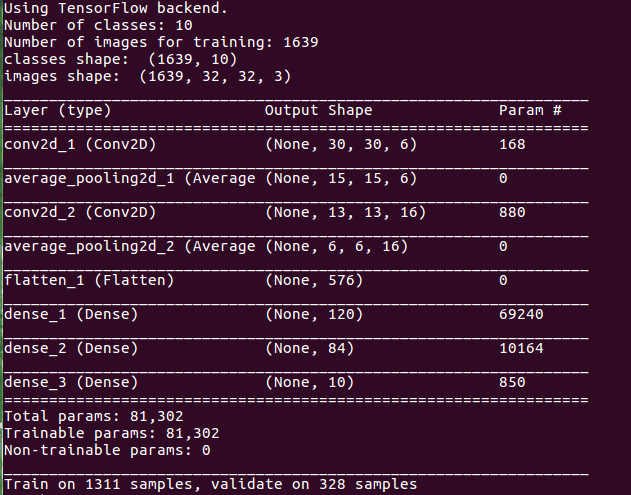
\includegraphics[scale=0.45]{leNet_arhitektura.png}
\end{center}
\caption{Slojevi modela leNet-5 neuronske mreže}
\label{fig:leNet_arh}
\end{figure}

Na slici \ref{fig:leNet_trening_acc} možemo videti da je preciznost na trening skupu u poslednje tri iteracije bila najveća moguća, tj 1.00. Na slici \ref{fig:leNet_test_acc} je prikazan rezultat rada modela na test podacima. Preciznost (\textit{accuracy}) iznosi 0.91. Takođe vidimo da je preciznost (\textit{precision}) za pojedinačne klase visoka. Na osnovu matrice konfuzije može se videti da veoma malo podataka pogrešno klasifikuje.


\begin{figure}[h!]
\begin{center}
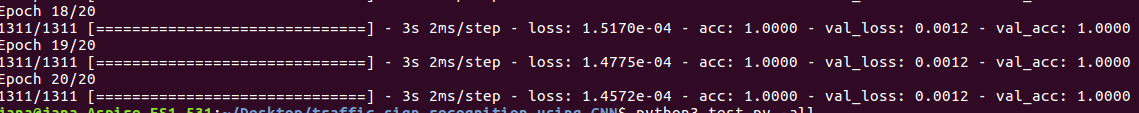
\includegraphics[scale=0.35]{leNet_trening_acc.png}
\end{center}
\caption{Preciznost na trening podecima}
\label{fig:leNet_trening_acc}
\end{figure}

\begin{figure}[h!]
\begin{center}
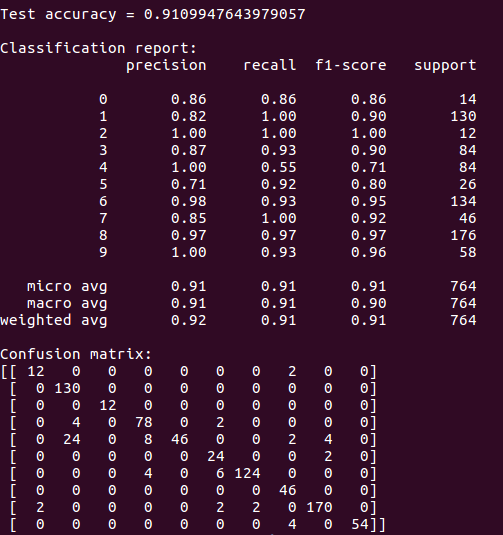
\includegraphics[scale=0.45]{leNet_test_acc.png}
\end{center}
\caption{Preciznost na test podecima}
\label{fig:leNet_test_acc}
\end{figure}




\newpage

\section{Zaključak}
\label{sec:zakljucak}

\newpage

\addcontentsline{toc}{section}{Literatura}
\appendix
\bibliography{seminarski} 
\bibliographystyle{plain}

\newpage

\appendix
%\section{Dodatak}
%\subsection{Dodatak 1}


\end{document}
